\documentclass[12pt]{article}
\usepackage[english]{babel}
\usepackage[utf8x]{inputenc}
\usepackage{amsmath}
\usepackage{graphicx}
\usepackage{caption}
\usepackage{booktabs}
\usepackage{float}
\usepackage[colorinlistoftodos]{todonotes}
\usepackage{subcaption}
\usepackage[colorlinks=true, linkcolor=blue]{hyperref}
\usepackage{array}
\usepackage{makecell}
\usepackage[margin=1in]{geometry}
\usepackage[most]{tcolorbox}
\setlength{\textfloatsep}{10pt plus 2pt minus 2pt}
\setlength{\floatsep}{8pt plus 2pt minus 2pt}
\setlength{\intextsep}{8pt plus 2pt minus 2pt}
\newtcolorbox{samplecalc}[1]{breakable, colback=gray!5, colframe=gray!55, boxrule=0.4pt, arc=1pt,
  left=8pt, right=8pt, top=4pt, bottom=2pt, title={#1}, fonttitle=\bfseries\small,
  coltitle=black, colbacktitle=gray!20, before skip=6pt, after skip=8pt, fontupper=\small,
  before upper={\setlength{\abovedisplayskip}{1pt}\setlength{\belowdisplayskip}{1pt}\setlength{\abovedisplayshortskip}{1pt}\setlength{\belowdisplayshortskip}{1pt}\setlength{\jot}{1.5pt}}}
\graphicspath{{./}{figures/}{../figures/}}

\newcolumntype{C}[1]{>{\centering\arraybackslash}p{#1}}
\bibliographystyle{ieeetr}


\begin{document}

\begin{titlepage}

\newcommand{\HRule}{\rule{\linewidth}{0.5mm}}

\center

\textsc{\LARGE University of Michigan}\\[1.5cm]
\textsc{\Large NERS 515}\\[0.5cm]
\textsc{\large Nuclear Measurements Laboratory}\\[0.5cm]

\HRule \\[0.4cm]
{ \huge \bfseries Laboratory 5: Proportional Counter}\\[0.4cm]
\HRule \\[0.7cm]

\Large \emph{Authors:}\\
Celing \textsc{Li}\\
Charalampos Alexander \textsc{Korfiatis}\\[0.7cm]

{\large October XX, 2026}\\[0.7cm] % TODO: set the submission date

\includegraphics[width=0.4\textwidth]{michigan_seal.png}\\[1cm]

\vfill

\end{titlepage}

\tableofcontents

\newpage

\begin{abstract}

\phantomsection
\addcontentsline{toc}{section}{Abstract}

% Written last by whoever finishes their part last.

\end{abstract}


\section{Introduction}

% PARTNER writes this section.


\section{Theory}

% PARTNER writes this section.


\section{Equipment and Procedure}

% PARTNER writes this section.


\section{Data}
\label{sec:data}

Count uncertainties are $\sigma_N = \sqrt{N}$ \cite{knoll}. All count times are Maestro live time, and we did not take a background count. The amplifier gain was 50 (coarse 100, fine 0.5) for the whole lab and the shaping time was 3~$\mu$s outside the shaping-time scan. We recorded the fine gain dial at 0.0, its 0.5$\times$ end, but it may have read 6.00, which would be a gain of about 110. No calculated result depends on the absolute gain, since it did not change during the lab.

\subsection{Shaping time}

Table~\ref{tab:rawshape} gives the Am-241 alpha peak centroid and gross area for each shaping time at 800~V, about 1 minute each \cite{labmanual}. The centroid rises from 1723 at 0.5~$\mu$s to 2422 at 10~$\mu$s. We did not record the area at 10~$\mu$s.

\begin{table}[!htbp]
\centering\small
\begin{tabular}{ccc}
\toprule
\textbf{Shaping time ($\mu$s)} & \textbf{Centroid (channel)} & \textbf{Gross area (counts)} \\
\midrule
0.5 & 1723.08 & 599257 $\pm$ 774 \\
1 & 2025.16 & 624639 $\pm$ 790 \\
2 & 2215.87 & 632332 $\pm$ 795 \\
3 & 2367.29 & 712298 $\pm$ 844 \\
6 & 2382.50 & 738092 $\pm$ 859 \\
10 & 2421.64 & not recorded \\
\bottomrule
\end{tabular}
\caption{Alpha peak centroid and gross area vs shaping time, Am-241 at 800~V.}
\label{tab:rawshape}
\end{table}

\subsection{Alpha counting curve}

Table~\ref{tab:rawalpha} lists the gross counts above LLD channel 1738 and the peak centroid, 30~s per point. The manual suggests 300--800~V \cite{labmanual}; we kept raising the voltage until the count rate leveled off. Counts first appeared at 400~V. At 1050~V the counts dropped from 669,674 to 286,105. We re-measured that point several times and got the same result, so we stopped there and took 1000~V as the start of the plateau. From 500 to 850~V the recorded centroid stays between 1744 and 2133, close to the LLD, and does not rise steadily. We did not save a sample spectrum (.SPE file), which the manual asks for \cite{labmanual}.

\begin{table}[!htbp]
\centering\small\setlength{\tabcolsep}{3pt}
\begin{tabular}{ccc|ccc}
\toprule
\textbf{HV (V)} & \textbf{Counts (30 s)} & \textbf{Centroid} & \textbf{HV (V)} & \textbf{Counts (30 s)} & \textbf{Centroid} \\
\midrule
300 & 0 $\pm$ 0 & -- & 725 & 121059 $\pm$ 348 & 1753.07 \\
400 & 23 $\pm$ 5 & -- & 750 & 224018 $\pm$ 473 & 1881.92 \\
500 & 398 $\pm$ 20 & 1777.10 & 775 & 294972 $\pm$ 543 & 2118.21 \\
550 & 2516 $\pm$ 50 & 1764.00 & 800 & 390186 $\pm$ 625 & 1743.68 \\
600 & 11163 $\pm$ 106 & 1760.00 & 850 & 563218 $\pm$ 750 & 2133.17 \\
625 & 19972 $\pm$ 141 & 1765.85 & 900 & 617516 $\pm$ 786 & 2738.47 \\
650 & 32190 $\pm$ 179 & 1754.00 & 1000 & 669674 $\pm$ 818 & 3232.47 \\
675 & 46571 $\pm$ 216 & 1822.40 & 1050 & 286105 $\pm$ 535 & 7166.13 \\
700 & 61980 $\pm$ 249 & 1784.90 & & & \\
\bottomrule
\end{tabular}
\caption{Alpha counting curve, Am-241: gross counts above LLD channel 1738 and peak centroid channel.}
\label{tab:rawalpha}
\end{table}

\subsection{Beta counting curve}

Table~\ref{tab:rawbeta} lists the Cl-36 counts above LLD channel 307, 30~s per point. Counts first appeared at 1100~V and we stopped at 1550~V. The centroid stays near the LLD (305--335) up to 1450~V, then reads 508 and 773.

\begin{table}[!htbp]
\centering\small
\begin{tabular}{ccc}
\toprule
\textbf{HV (V)} & \textbf{Counts (30 s)} & \textbf{Centroid} \\
\midrule
1000 & 0 $\pm$ 0 & -- \\
1100 & 23161 $\pm$ 152 & 328.36 \\
1200 & 97809 $\pm$ 313 & 334.88 \\
1300 & 242325 $\pm$ 492 & 304.65 \\
1400 & 345372 $\pm$ 588 & 311.34 \\
1450 & 521827 $\pm$ 722 & 320.22 \\
1500 & 664725 $\pm$ 815 & 507.70 \\
1550 & 692883 $\pm$ 832 & 773.28 \\
\bottomrule
\end{tabular}
\caption{Beta counting curve, Cl-36: gross counts above LLD channel 307 and centroid channel.}
\label{tab:rawbeta}
\end{table}

\subsection{Absolute efficiency}

We counted the Cl-36 source for 60~s at 1500~V, picked from the beta counting curve, with the same LLD (307) and gain: $1{,}428{,}191 \pm 1195$ counts. The source was marked 1.032~$\mu$Ci on August 1, 2026.

\subsection{Gamma response}

Table~\ref{tab:rawgamma} lists the counts with the Co-60 source turned upside down to block the betas \cite{labmanual}, LLD channel 229, 30~s per point. The counts rise to about 51,000 at 1500--1600~V and then fall at 1650 and 1700~V. We did not notice anything unusual at the time.

\begin{table}[!htbp]
\centering\small
\begin{tabular}{cc|cc}
\toprule
\textbf{HV (V)} & \textbf{Counts (30 s)} & \textbf{HV (V)} & \textbf{Counts (30 s)} \\
\midrule
1000 & 0 $\pm$ 0 & 1550 & 50648 $\pm$ 225 \\
1200 & 10490 $\pm$ 102 & 1600 & 51362 $\pm$ 227 \\
1300 & 24776 $\pm$ 157 & 1650 & 48634 $\pm$ 221 \\
1400 & 43711 $\pm$ 209 & 1700 & 43041 $\pm$ 207 \\
1500 & 51324 $\pm$ 227 & & \\
\bottomrule
\end{tabular}
\caption{Gamma response, Co-60 turned upside down: gross counts above LLD channel 229.}
\label{tab:rawgamma}
\end{table}

\section{Analysis of Data}
\label{sec:analysis}

A rate from $N$ counts in time $t$ is $r = N/t$ with $\sigma_r = \sqrt{N}/t$ (Knoll, Eq.~3.40) \cite{knoll}. Other uncertainties are propagated with Knoll Eq.~3.37.

\subsection{Shaping time and ballistic deficit}

The ballistic deficit is the amplitude lost because the shaping time is too short to follow the whole pulse rise (Knoll, p.~649, Fig.~17.22) \cite{knoll}. Relative to 10~$\mu$s,
\begin{equation}
\text{BD} = \frac{C_{10} - C}{C_{10}} \times 100\%,
\end{equation}
with $C$ the centroid channel. The statistical uncertainty of a peak centroid is (Knoll, p.~728)
\begin{equation}
\sigma_c = \frac{\text{FWHM}/2.35}{\sqrt{A}},
\end{equation}
with $A$ the peak area. We did not record the FWHM, so we cannot evaluate this. With $A \approx 6$--$7 \times 10^5$ counts, even a peak several hundred channels wide gives $\sigma_c$ below one channel, so we use $\sigma_c = 1$ channel as an upper bound. This only covers counting statistics, not the ROI placement or gain drift (Section~\ref{sec:amp}). The 10~$\mu$s area, which we did not record, is estimated as $7.7 \times 10^5$ counts from a line through the 3 and 6~$\mu$s areas; it only enters $\sigma_c$.

\begin{samplecalc}{Sample calculation: ballistic deficit at 0.5 $\mu$s ($C = 1723.08$, $C_{10} = 2421.64$, $\sigma_c = 1$)}
\begin{align*}
\text{BD} &= \frac{2421.64 - 1723.08}{2421.64} \times 100\% = 28.85\%\\
\sigma_{\text{BD}} &= 100\%\,\sigma_c\sqrt{\left(\frac{1}{C_{10}}\right)^2 + \left(\frac{C}{C_{10}^2}\right)^2}
 = 100\%\sqrt{(4.13\times10^{-4})^2 + (2.94\times10^{-4})^2} = 0.05\%
\end{align*}
\end{samplecalc}

\begin{figure}[!htbp]
\centering
\begin{minipage}[c]{0.38\textwidth}\centering\small
\begin{tabular}{cc}
\toprule
\textbf{Shaping ($\mu$s)} & \textbf{BD (\%)} \\
\midrule
0.5 & 28.85 $\pm$ 0.05 \\
1 & 16.37 $\pm$ 0.05 \\
2 & 8.50 $\pm$ 0.06 \\
3 & 2.24 $\pm$ 0.06 \\
6 & 1.62 $\pm$ 0.06 \\
\bottomrule
\end{tabular}
\captionof{table}{Ballistic deficit relative to 10~$\mu$s.}
\label{tab:bd}
\end{minipage}\hfill
\begin{minipage}[c]{0.58\textwidth}\centering
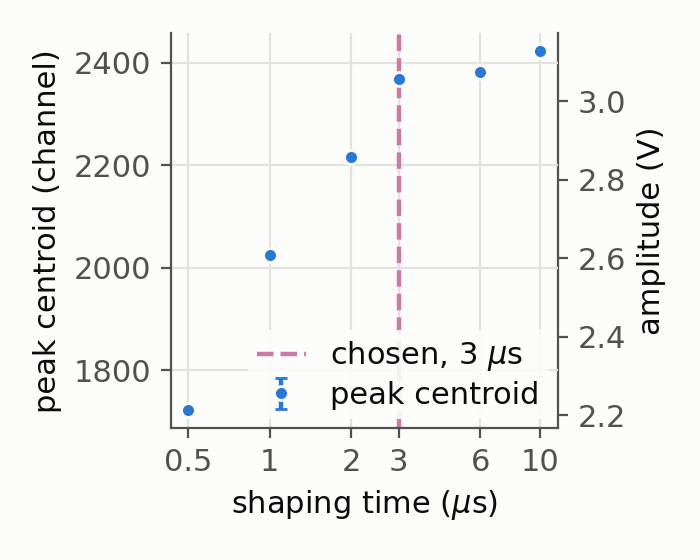
\includegraphics[width=\textwidth]{F1_centroid_vs_shaping_time.png}
\captionof{figure}{Alpha peak centroid vs shaping time; dashed line: chosen 3~$\mu$s. Error bars ($\pm$1 channel, upper bound) are smaller than the markers.}
\label{fig:shaping}
\end{minipage}
\end{figure}

Figure~\ref{fig:shaping} shows the centroid climbing steeply up to 3~$\mu$s and then leveling off. The deficit is 28.85~$\pm$~0.05\% at 0.5~$\mu$s and 2.24~$\pm$~0.06\% at 3~$\mu$s (Table~\ref{tab:bd}); going on to 6~$\mu$s only recovers another 0.6\%. We chose 3~$\mu$s as the shortest shaping time without a significant deficit, as the manual asks \cite{labmanual}.

This follows from the pulse shape. Most of the signal comes from the positive ions drifting away from the anode wire. The pulse reaches half its height in about 0.25\% of the full ion collection time, but the full collection takes several hundred microseconds (Knoll, Eqs.~6.35 and 6.38, pp.~181--182). A shaping time of a few microseconds cuts off the slow remainder, and the shorter it is, the more amplitude is lost. Knoll recommends shaping times of several microseconds for proportional counters, long compared with the spread in pulse rise times (p.~183). We did not measure the rise time of the amplifier output on the scope. A longer shaping time gives an output pulse that rises more slowly and peaks later, with an amplitude closer to the full value (lecture slides, Ch.~16--17, slide 50).

\subsection{Alpha counting curve}

Table~\ref{tab:alpharate} gives the rates near the plateau (all rates are in Appendix~\ref{app:rates}) and Figure~\ref{fig:alphacc} shows the counting curve. We quote the plateau slope as the percent change in rate per 100~V, relative to the rate at the start of the range \cite{knoll}.

\begin{samplecalc}{Sample calculation: rate at 1000 V and plateau slope over 900--1000 V}
\begin{align*}
r_{1000} &= 669674/(30\ \text{s}) = 22322\ \text{s}^{-1}, & \sigma &= \sqrt{669674}/(30\ \text{s}) = 27\ \text{s}^{-1}\\
r_{900} &= 617516/(30\ \text{s}) = 20584\ \text{s}^{-1}, & \sigma &= \sqrt{617516}/(30\ \text{s}) = 26\ \text{s}^{-1}
\end{align*}
\begin{align*}
s_{\%} &= 100\,\frac{r_{1000} - r_{900}}{r_{900}} = 100\,\frac{1738.6}{20584} = 8.4\%\ \text{per 100 V},\\
\sigma_{s_\%} &= 100\,\frac{\sqrt{26^2 + 27^2}}{20584} = 0.2\%\ \text{per 100 V}
\end{align*}
\end{samplecalc}

\begin{figure}[!htbp]
\centering
\begin{minipage}[c]{0.36\textwidth}\centering\small
\begin{tabular}{cc}
\toprule
\textbf{HV (V)} & \textbf{Rate (s$^{-1}$)} \\
\midrule
850 & 18774 $\pm$ 25 \\
900 & 20584 $\pm$ 26 \\
1000 & 22322 $\pm$ 27 \\
1050 & 9537 $\pm$ 18 \\
\bottomrule
\end{tabular}
\captionof{table}{Alpha count rates near the plateau.}
\label{tab:alpharate}
\end{minipage}\hfill
\begin{minipage}[c]{0.60\textwidth}\centering
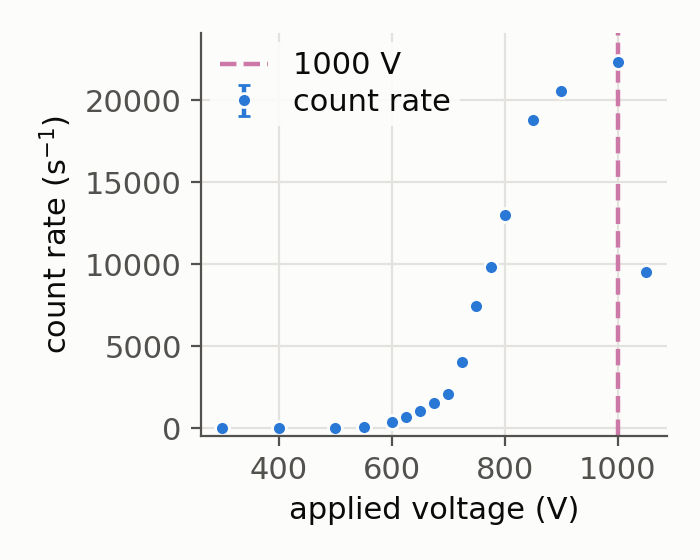
\includegraphics[width=\textwidth]{F2_alpha_counting_curve_lin.png}
\captionof{figure}{Alpha counting curve, Am-241, LLD channel 1738; dashed line: 1000~V, start of the plateau. Error bars ($\sqrt{N}/t$) are smaller than the markers.}
\label{fig:alphacc}
\end{minipage}
\end{figure}

Knoll's expected curve has no counts until the alpha pulses clear the LLD, a steep rise as the alpha peak crosses it, then a flat plateau once every alpha is counted (Knoll, pp.~113--115, 185). Ours has the rise, from 400 to 850~V, but flattens only over 900--1000~V, with a slope of 8.4~$\pm$~0.2\% per 100~V. So the plateau is barely established and not flat.

The drop to 9537~s$^{-1}$ at 1050~V is not expected. Past the plateau the rate should stay flat or climb as spurious pulses start to be counted (Knoll, p.~184). The counts were taken in live time, which corrects for the MCA dead time, so dead time is not the cause. Possible causes:
\begin{itemize}
\item amplifier saturation, which the manual warns about at high voltage \cite{labmanual};
\item pulses pushed past the top MCA channel and not recorded, since the centroid at 1050~V is already at channel 7166 (our inference);
\item pile-up: at about $2\times10^4$~s$^{-1}$ with pulses several microseconds wide, the duty cycle (pulse width $\times$ rate) approaches the $10^{-1}$ that Knoll calls a high-rate situation (p.~648), and live time does not correct for pile-up.
\end{itemize}
We left 1050~V out of the plateau and took 1000~V as its start. No later section uses the alpha operating point, so the drop does not affect the other results.

\subsection{Alpha pulse amplitude vs voltage}
\label{sec:amp}

The pulse charge is $Q = n_0 e M$ (Knoll, Eq.~6.6), and by the Diethorn model (Knoll, Eq.~6.10) $\ln M$ grows roughly linearly with $V$ (p.~171). So the centroid on a log axis vs voltage should follow a straight line, the trend of Knoll Fig.~6.11. We compare neighbouring points with the two-point slope $s = \ln(C_2/C_1)/\Delta V$.

\begin{samplecalc}{Sample calculation: two-point slope, 900--1000 V ($C_1 = 2738.47$, $C_2 = 3232.47$, $\sigma_c = 1$)}
\begin{align*}
s &= \frac{\ln(3232.47/2738.47)}{100\ \text{V}} = 1.66\times10^{-3}\ \text{V}^{-1},\\
\sigma_s &= \frac{\sqrt{(1/2738.47)^2 + (1/3232.47)^2}}{100\ \text{V}} = 5\times10^{-6}\ \text{V}^{-1}
\end{align*}
The same for 1000--1050 V gives $s = (1.592 \pm 0.001)\times10^{-2}$ V$^{-1}$.
\end{samplecalc}

\begin{figure}[!htbp]
\centering
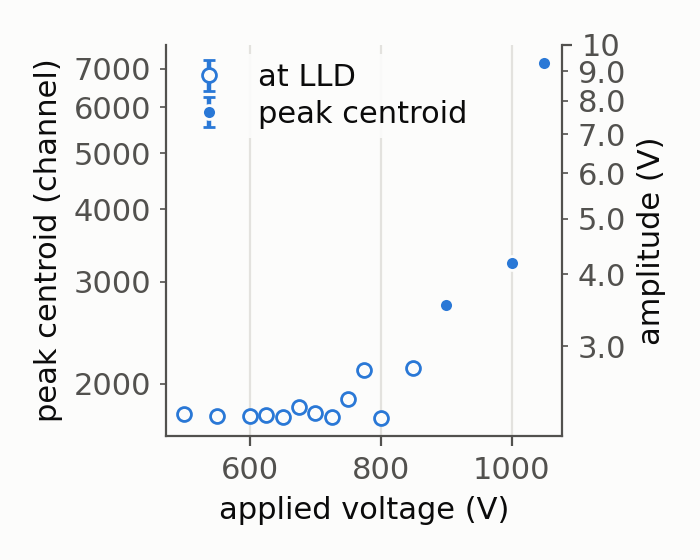
\includegraphics[width=0.55\textwidth]{F3_alpha_amplitude_vs_voltage_with_low.png}
\caption{Alpha peak centroid vs voltage on a log axis. Hollow: 500--850~V, where the centroid sits at the LLD. Error bars ($\pm$1 channel) are smaller than the markers.}
\label{fig:amp}
\end{figure}

From 500 to 850~V the centroid stays within a few hundred channels of the LLD (hollow points in Figure~\ref{fig:amp}). In this range the alpha peak was either below the LLD with only its upper edge counted, or not yet separated from the noise. Either way the number is the centroid of the counts above the LLD, not of the peak, so we leave these points out. This does not affect the counting curve, which only uses counts above the LLD; that range is where the alpha pulses cross the LLD.

That leaves 900, 1000 and 1050~V, and the 1050~V point is suspect (previous section). The two slopes differ by about a factor of ten, so we cannot confirm the straight-line trend of Fig.~6.11 from our data. For scale, Knoll's P-10 example gives a 17.4\% increase in $M$ for a 1\% increase in $V$ at 1793~V (Table~6.3, p.~178), or $\ln(1.174)/17.9\ \text{V} = 9\times10^{-3}$~V$^{-1}$, between our two values. Fig.~6.11 is for xenon mixtures (p.~170), so only the trend compares.

The gain also drifted. In the shaping-time scan the peak sat at channel 2367 at 800~V (3~$\mu$s), but on the counting curve at the same voltage and amplifier gain the centroid was at the LLD. So the gas multiplication changed between the two sections. Knoll notes that pressure changes of a few tenths of a percent matter in flow counters and that $M$ falls about 8.6\% for a 1\% rise in pressure; HV changes of 0.1--0.2\% also matter (p.~178, Table~6.3). We had turned the gas flow to maximum at the start \cite{labmanual}.

\subsection{Energy calibration and spectrum}

We did not save a spectrum, so we cannot show the calibrated alpha spectrum or identify its features from data. We can still calibrate from a centroid. Am-241 emits alphas at 5.486~MeV (85.2\%) and 5.443~MeV (12.8\%) (Knoll, Table~1.3, p.~8), which our counter does not resolve, so we assign 5.486~MeV to the peak. With one peak, we assume the linear calibration passes through the origin, $E = k \times \text{channel}$ (our assumption). We use the 3~$\mu$s shaping-time run, where the ROI was drawn around the whole peak.

\begin{samplecalc}{Sample calculation: calibration factor (800 V, gain 50, 3 $\mu$s, $C = 2367.29$)}
\begin{align*}
k &= \frac{5486\ \text{keV}}{2367.29} = 2.317\ \text{keV/channel}, &
\sigma_k &= k\,\frac{\sigma_c}{C} = 2.317\,\frac{1}{2367.29} = 0.001\ \text{keV/channel}
\end{align*}
\end{samplecalc}

This factor holds only at 800~V, gain 50, 3~$\mu$s shaping, and the gas gain during the shaping-time runs. The same calculation at 1000~V on the counting curve would give 1.70~keV/channel. Without the measured spectrum, we can only describe what Knoll predicts: one roughly Gaussian alpha peak, since the alphas stop in the gas, plus noise and single-ion-pair events at low pulse height, below the LLD (Knoll, pp.~175, 185).

\subsection{Beta counting curve}

Figure~\ref{fig:bg} shows the Cl-36 beta counting curve with the gamma curve; the rates are in Appendix~\ref{app:rates}.

\begin{samplecalc}{Sample calculation: rate at 1500 V and plateau slope over 1500--1550 V}
\begin{align*}
r_{1500} &= 664725/(30\ \text{s}) = 22158\ \text{s}^{-1}, & \sigma &= 27\ \text{s}^{-1}\\
r_{1550} &= 692883/(30\ \text{s}) = 23096\ \text{s}^{-1}, & \sigma &= 28\ \text{s}^{-1}
\end{align*}
\begin{align*}
s_{\%} &= 100\,\frac{r_{1550} - r_{1500}}{r_{1500}}\cdot\frac{100\ \text{V}}{50\ \text{V}} = 8.5\%\ \text{per 100 V},\\
\sigma_{s_\%} &= 100\,\frac{\sqrt{27^2 + 28^2}}{22158}\cdot 2 = 0.4\%\ \text{per 100 V}
\end{align*}
\end{samplecalc}

\begin{figure}[!htbp]
\centering
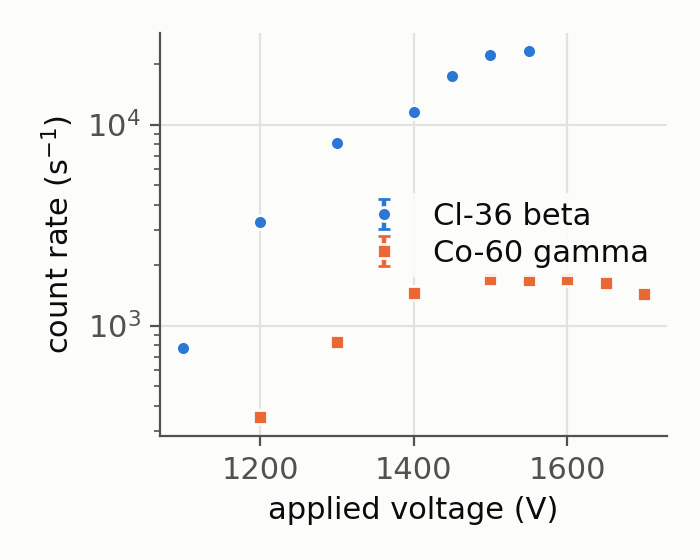
\includegraphics[width=0.55\textwidth]{F5_beta_gamma_counting_curves.png}
\caption{Counting curves for Cl-36 betas (LLD channel 307) and Co-60 gammas (LLD channel 229). Error bars ($\sqrt{N}/t$) are smaller than the markers.}
\label{fig:bg}
\end{figure}

Knoll expects a beta counting curve that rises more gradually than the alpha curve and has a shorter, more sloped plateau, because the beta pulse heights are spread out and sit close to the noise (Knoll, p.~186). Ours rises over 1100--1500~V and flattens only between 1500 and 1550~V, with a slope of 8.5~$\pm$~0.4\% per 100~V. We stopped at 1550~V, so we cannot say how long the plateau is.

The beta pulses are much smaller than the alpha pulses. At the same amplifier gain, alpha pulses cleared an LLD of channel 1738 from 400--500~V, while beta pulses needed 1100~V to clear channel 307, and the beta centroid stayed at the LLD up to 1450~V. A beta's range is much longer than the chamber, so it loses only a small part of its energy in the gas, while an alpha stops in the gas and deposits all of it (Knoll, p.~185).

\subsection{Absolute and intrinsic efficiency}

The absolute efficiency is the number of pulses recorded per particle emitted, and the intrinsic efficiency is per particle that enters the detector. For an isotropic source they are related by the solid angle $\Omega$ (Knoll, Eqs.~4.16--4.17, pp.~118--119) \cite{knoll}:
\begin{equation}
\varepsilon_{\text{abs}} = \frac{r}{A}, \qquad \varepsilon_{\text{int}} = \varepsilon_{\text{abs}}\,\frac{4\pi}{\Omega},
\end{equation}
with $\Omega = 2\pi$ for our counter (Knoll, p.~166). The activity on the day of the measurement is $A = A_0 e^{-\lambda t}$ with $\lambda = \ln 2/T_{1/2}$ (Knoll, Eq.~1.1, p.~2) and $T_{1/2} = 3.08\times10^5$~y for Cl-36 (Knoll, Table~1.1, p.~4), so the decay since August 1 is negligible. The marked activity has no stated uncertainty, so the quoted uncertainties are from counting only.

\begin{samplecalc}{Sample calculation: efficiency}
\begin{align*}
r &= 1428191/(60\ \text{s}) = 23803\ \text{s}^{-1}, & \sigma_r &= \sqrt{1428191}/(60\ \text{s}) = 20\ \text{s}^{-1}\\
A &= 1.032\ \mu\text{Ci} \times 3.7\times10^{4}\ \text{Bq}/\mu\text{Ci} = 38184\ \text{Bq} & &\\
\varepsilon_{\text{abs}} &= 23803/38184 = 0.6234, & \sigma &= 0.6234 \times 20/23803 = 0.0005\\
\varepsilon_{\text{int}} &= 0.6234 \times 4\pi/2\pi = 1.247, & \sigma &= 0.001
\end{align*}
\end{samplecalc}

\begin{table}[!htbp]
\centering\small
\begin{tabular}{lc}
\toprule
\textbf{Quantity} & \textbf{Value} \\
\midrule
Count rate $r$ (s$^{-1}$) & 23803 $\pm$ 20 \\
Activity $A$ (Bq) & 38184 \\
$\varepsilon_{\text{abs}}$ & 0.6234 $\pm$ 0.0005 \\
$\varepsilon_{\text{int}}$ ($\Omega = 2\pi$) & 1.247 $\pm$ 0.001 \\
\bottomrule
\end{tabular}
\caption{Absolute and intrinsic efficiency, Cl-36 at 1500~V (counting uncertainty only).}
\label{tab:eff}
\end{table}

For 2$\pi$ geometry the absolute efficiency should be at most about 0.5, and the intrinsic efficiency for betas about 100\% on the plateau, since every charged particle that enters the gas makes a pulse (Knoll, pp.~118, 166, 185). We measured $\varepsilon_{\text{abs}} = 0.6234 \pm 0.0005$ and $\varepsilon_{\text{int}} = 1.247 \pm 0.001$ (Table~\ref{tab:eff}). An intrinsic efficiency above 100\% is not physical, so the intrinsic efficiency is not as expected: something added counts, or the reference activity is too low for our source. Likely sources:
\begin{itemize}
\item betas emitted into the source backing can backscatter and come back out of the source surface, which raises the apparent beta yield (Knoll, p.~46);
\item the gain drifted: at the same 1500~V, LLD and gain, the rate was 7.4~$\pm$~0.2\% higher than on the beta counting curve (22158~s$^{-1}$), which matches the gas-gain drift in Section~\ref{sec:amp} (Knoll, p.~178);
\item spurious afterpulses become more likely at high gas multiplication (Knoll, p.~184);
\item we did not take a background count;
\item the marked activity has no stated uncertainty.
\end{itemize}
Self-absorption in the source and a solid angle below 2$\pi$ would lower the efficiency (Knoll, p.~185), so they cannot explain a value that is too high. We chose 1500~V from the plateau of the beta counting curve, which is the usual way to pick an operating point (Knoll, p.~185), but it sits at the very start of a short plateau.

\subsection{Gamma response}

\begin{samplecalc}{Sample calculation: gamma rate at 1500 V and plateau slope over 1500--1600 V}
\begin{align*}
r_{1500} &= 51324/(30\ \text{s}) = 1710.8\ \text{s}^{-1}, & \sigma &= \sqrt{51324}/(30\ \text{s}) = 7.6\ \text{s}^{-1}\\
s_{\%} &= 100\,\frac{1712.1 - 1710.8}{1710.8} = 0.1\%\ \text{per 100 V}, & \sigma_{s_\%} &= 100\,\frac{\sqrt{7.6^2 + 7.6^2}}{1710.8} = 0.6\%\ \text{per 100 V}
\end{align*}
\end{samplecalc}

A gas counter is expected to respond weakly to gamma rays. The chance of a gamma interacting in the gas falls quickly with energy (Knoll, Fig.~6.18, p.~187), and most counts come from interactions in the counter wall whose electrons reach the gas, with an intrinsic efficiency of only about a percent (Knoll, p.~188). Our Co-60 rate peaks at about 1710~s$^{-1}$, against about 22000~s$^{-1}$ for Cl-36 betas at the same voltage; the sources differ, so this is not an efficiency ratio. Because those electrons lose different amounts of energy before reaching the gas (p.~188), we expected a broad pulse-height spread and a gradual curve like the beta one. The curve in Figure~\ref{fig:bg} rises from 1200~V and is flat over 1500--1600~V (0.1~$\pm$~0.6\% per 100~V), then falls by 16\% by 1700~V. We did not notice anything at the time; it may be the same high-voltage effect as the alpha drop (our inference).


\section{Conclusions}
\label{sec:conclusions}

The ballistic deficit relative to 10~$\mu$s was 28.85~$\pm$~0.05\% at 0.5~$\mu$s and 2.24~$\pm$~0.06\% at 3~$\mu$s. The centroid levels off from 3~$\mu$s, so 3~$\mu$s is the shortest shaping time without a significant deficit.

The alpha counting curve rose as expected and reached a short plateau from 1000~V, with a slope of 8.4~$\pm$~0.2\% per 100~V. The count rate then dropped by more than half at 1050~V, which Knoll's counting curve does not predict; amplifier saturation, pulses past the top MCA channel or pile-up could explain it.

The alpha pulse amplitude grew steeply with voltage, but the two usable slopes, $1.66\times10^{-3}$ and $1.59\times10^{-2}$~V$^{-1}$, differ by a factor of ten. With so few usable points we cannot confirm the straight-line trend of Knoll Fig.~6.11, and the gas gain drifted between sections.

The energy calibration factor is 2.317~$\pm$~0.001~keV/channel at 800~V, gain 50 and 3~$\mu$s. We did not save a spectrum, so we cannot show the calibrated spectrum.

The beta counting curve had a short, sloped plateau (8.5~$\pm$~0.4\% per 100~V), and beta pulses were much smaller than alpha pulses, both as Knoll predicts.

The absolute efficiency was 0.6234~$\pm$~0.0005 and the intrinsic efficiency 1.247~$\pm$~0.001, above the 0.5 and 100\% limits. The intrinsic efficiency is therefore not as expected; backscattering from the source backing and gain drift are the most likely causes.

The gamma rate from Co-60 peaked at 1712~$\pm$~8~s$^{-1}$, low as expected for a gas counter, with a flat region over 1500--1600~V and a drop at higher voltage.

\bibliography{references}

\appendix
\section{Count rates}
\label{app:rates}

\begin{table}[!htbp]
\centering\small\setlength{\tabcolsep}{4pt}
\begin{tabular}{cc|cc}
\toprule
\textbf{HV (V)} & \textbf{Rate (s$^{-1}$)} & \textbf{HV (V)} & \textbf{Rate (s$^{-1}$)} \\
\midrule
300 & 0.00 $\pm$ 0.00 & 725 & 4035.3 $\pm$ 11.6 \\
400 & 0.77 $\pm$ 0.16 & 750 & 7467.3 $\pm$ 15.8 \\
500 & 13.27 $\pm$ 0.66 & 775 & 9832.4 $\pm$ 18.1 \\
550 & 83.9 $\pm$ 1.7 & 800 & 13006.2 $\pm$ 20.8 \\
600 & 372.1 $\pm$ 3.5 & 850 & 18773.9 $\pm$ 25.0 \\
625 & 665.7 $\pm$ 4.7 & 900 & 20583.9 $\pm$ 26.2 \\
650 & 1073.0 $\pm$ 6.0 & 1000 & 22322.5 $\pm$ 27.3 \\
675 & 1552.4 $\pm$ 7.2 & 1050 & 9536.8 $\pm$ 17.8 \\
700 & 2066.0 $\pm$ 8.3 & & \\
\bottomrule
\end{tabular}
\caption{Alpha count rates, $r = N/30$~s, $\sigma_r = \sqrt{N}/30$~s.}
\label{tab:appalpha}
\end{table}

\begin{table}[!htbp]
\centering\small
\begin{tabular}{ccc}
\toprule
\textbf{HV (V)} & \textbf{Cl-36 beta (s$^{-1}$)} & \textbf{Co-60 gamma (s$^{-1}$)} \\
\midrule
1000 & 0.0 $\pm$ 0.0 & 0.0 $\pm$ 0.0 \\
1100 & 772.0 $\pm$ 5.1 & -- \\
1200 & 3260.3 $\pm$ 10.4 & 349.7 $\pm$ 3.4 \\
1300 & 8077.5 $\pm$ 16.4 & 825.9 $\pm$ 5.2 \\
1400 & 11512.4 $\pm$ 19.6 & 1457.0 $\pm$ 7.0 \\
1450 & 17394.2 $\pm$ 24.1 & -- \\
1500 & 22157.5 $\pm$ 27.2 & 1710.8 $\pm$ 7.6 \\
1550 & 23096.1 $\pm$ 27.7 & 1688.3 $\pm$ 7.5 \\
1600 & -- & 1712.1 $\pm$ 7.6 \\
1650 & -- & 1621.1 $\pm$ 7.4 \\
1700 & -- & 1434.7 $\pm$ 6.9 \\
\bottomrule
\end{tabular}
\caption{Beta and gamma count rates, $r = N/30$~s, $\sigma_r = \sqrt{N}/30$~s.}
\label{tab:appbg}
\end{table}

\end{document}
